\chapter{The South African energy sector}
The Republic of South Africa (SA) is one of the most developed country in Sub-Saharan Africa and acording to the Human Development Index (HDI) it is growing constand since the 1980's, nevertheless it counts as medium developed country \cite{UNDP2014}. Also the population and energy demand is constantly growing \cite{TheWorldBank2015,Agency2015}.

SA has also one of the strongest econemys in Africa, therefore it is accounting for about 30~\% of the primary energy consumption of the entire continent Africa in 2014 \cite{BP2015b}. 
\section{Primary energy consumption}
\begin{figure}[!b]
        \centering                
        \begin{subfigure}[b]{0.45\textwidth}
                \centering
                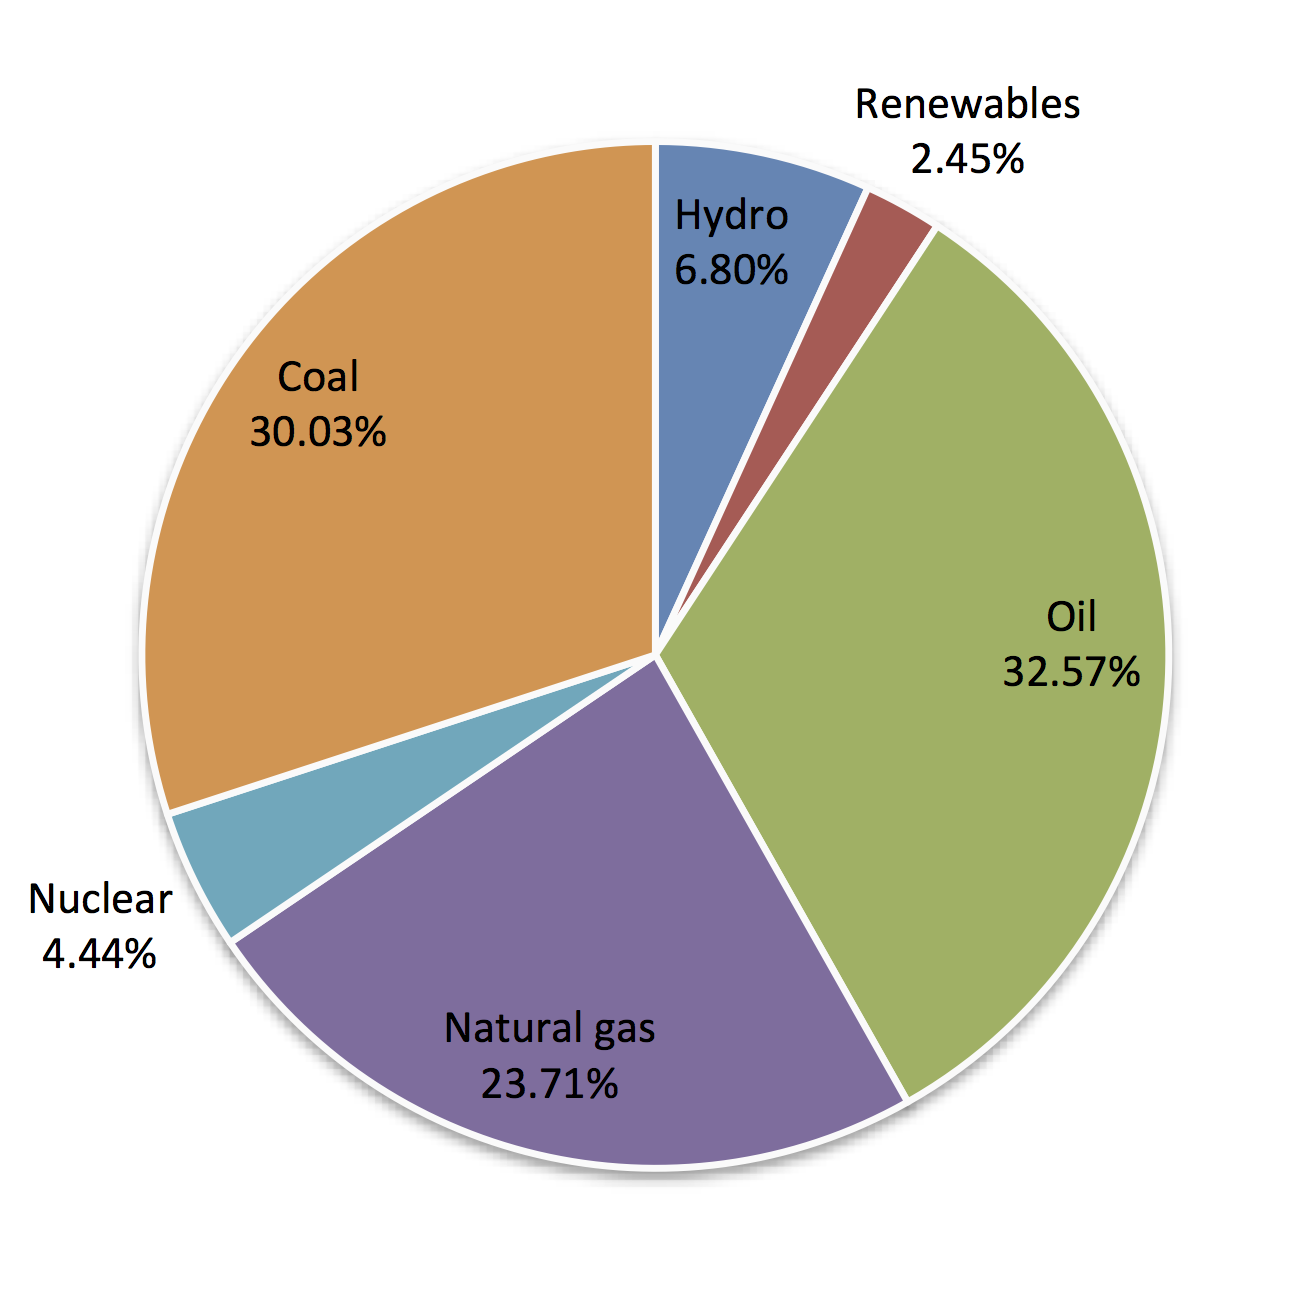
\includegraphics[width=1\textwidth]{FIG/PrimWorld}
                \caption{Worldwide allocation of primary energy consuption.}\label{PrimWorld}
        \end{subfigure}
        ~
        \begin{subfigure}[b]{0.45\textwidth}
                \centering
                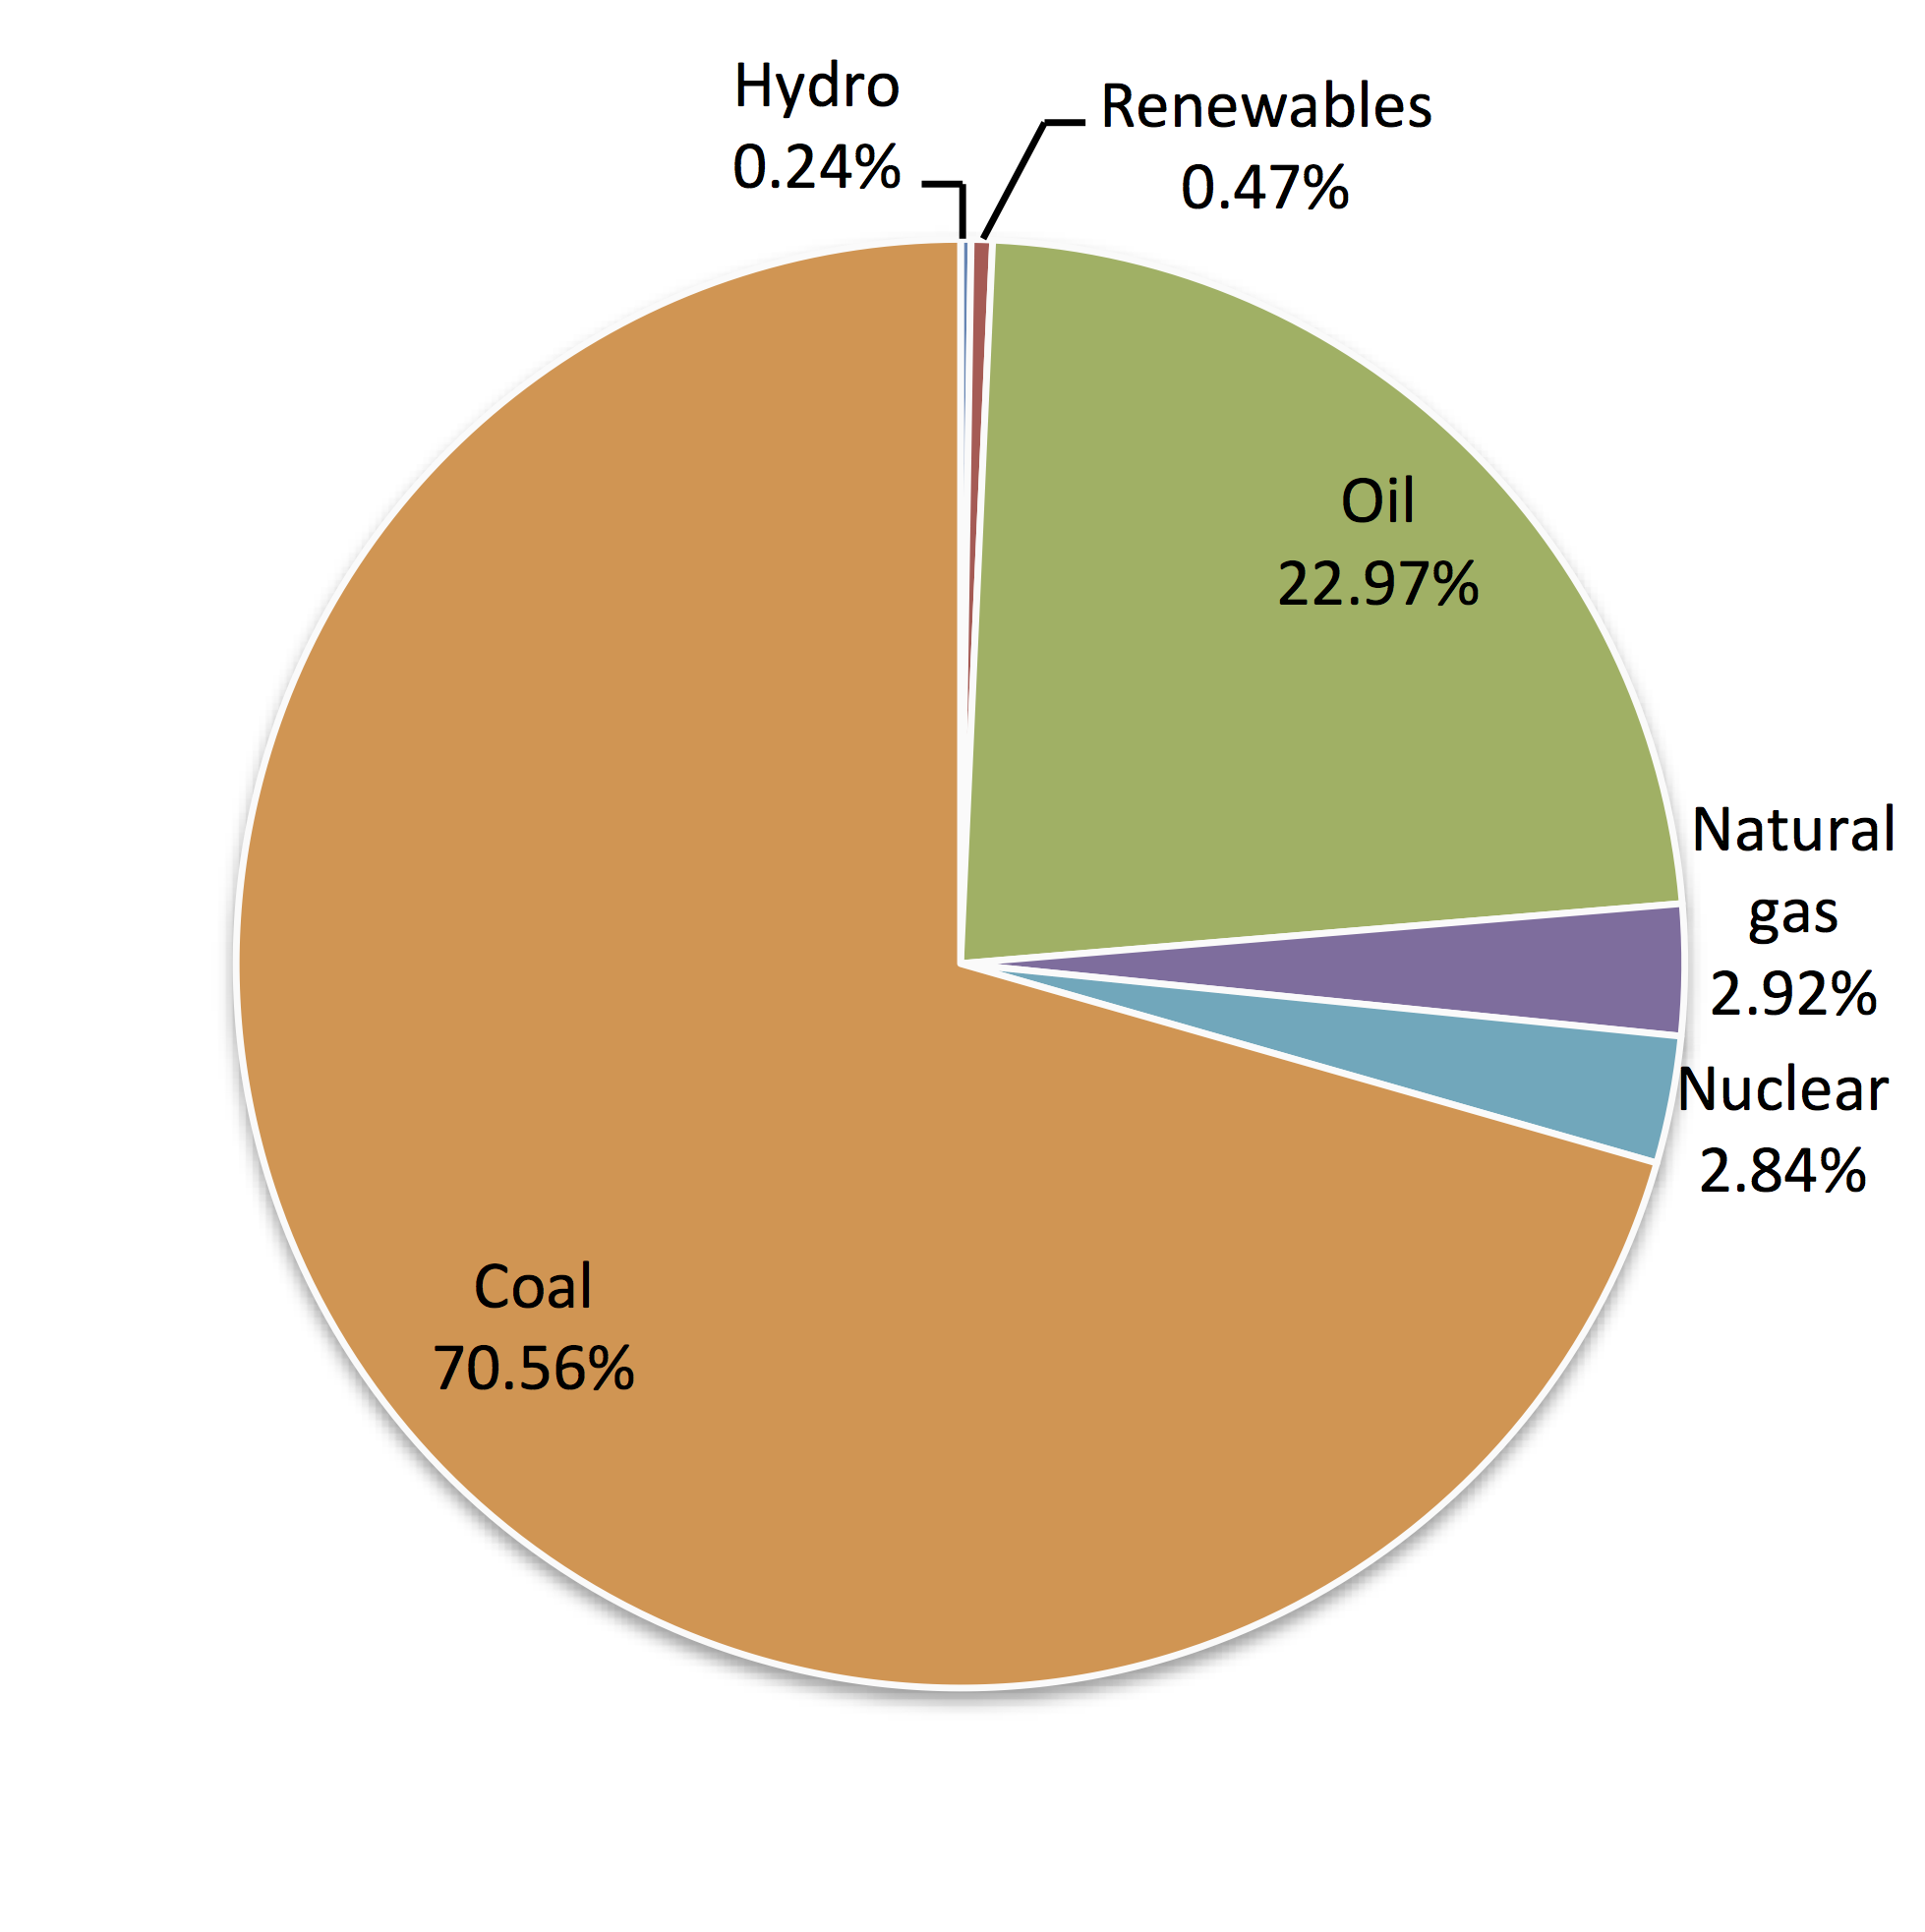
\includegraphics[width=1\textwidth]{FIG/PrimSA}
                \caption{SA's allocation of primary energy consuption.}\label{PrimSA}
        \end{subfigure}
\caption[Comparision of primary energy consumption by fuel in 2014.]{Comparision of primary energy consumption by fuel (excl. biomass and waste) in 2014 \cite{BP2015b}.}\label{PEKreis}
\end{figure}
The primary energy consumption of SA was in 2014 about 1~473.52~TWh \cite{BP2015b}. This consumption is mainly based on fossil energy resources. More than 96~\% of the primary energy consumption was in 2014 based fossil fuels and further 2.8~\% on nuclear. Thereby is the share on primary energy consumption predominant coming from coal. Figure \ref{PEKreis} shows the primary energy mix of SA in comparision with the worldwide primary energy mix. \cite{BP2015b}

It can be seen that coal is with about 71~\% the main primary energy source. Also crude oil (23~\%) is a very important energy source for SA. Therefor is the primary energy consumption from renewable energies in SA just about 0.7~\%. Comparing to this, the global share of  renewable primary energy consumption was about 9.3~\% in 2015. But it must be said that the share on renewable energy growth almost five times from 2013 to 2014. \cite{BP2015b}

Figure \ref{PrimEnergyDevelopment} shows the growing South African primary energy consumption. Between 1965 and 2014 the annual primary energy consumption in SA has risen from 351.96~TWh up to 1~473.52~TWh. Consequently a avarage anual growing rate in primary energy consumption in SA of 8.5~\% in the past half century. \cite{BP2015c}

\begin{figure}[htbp]  
\centering
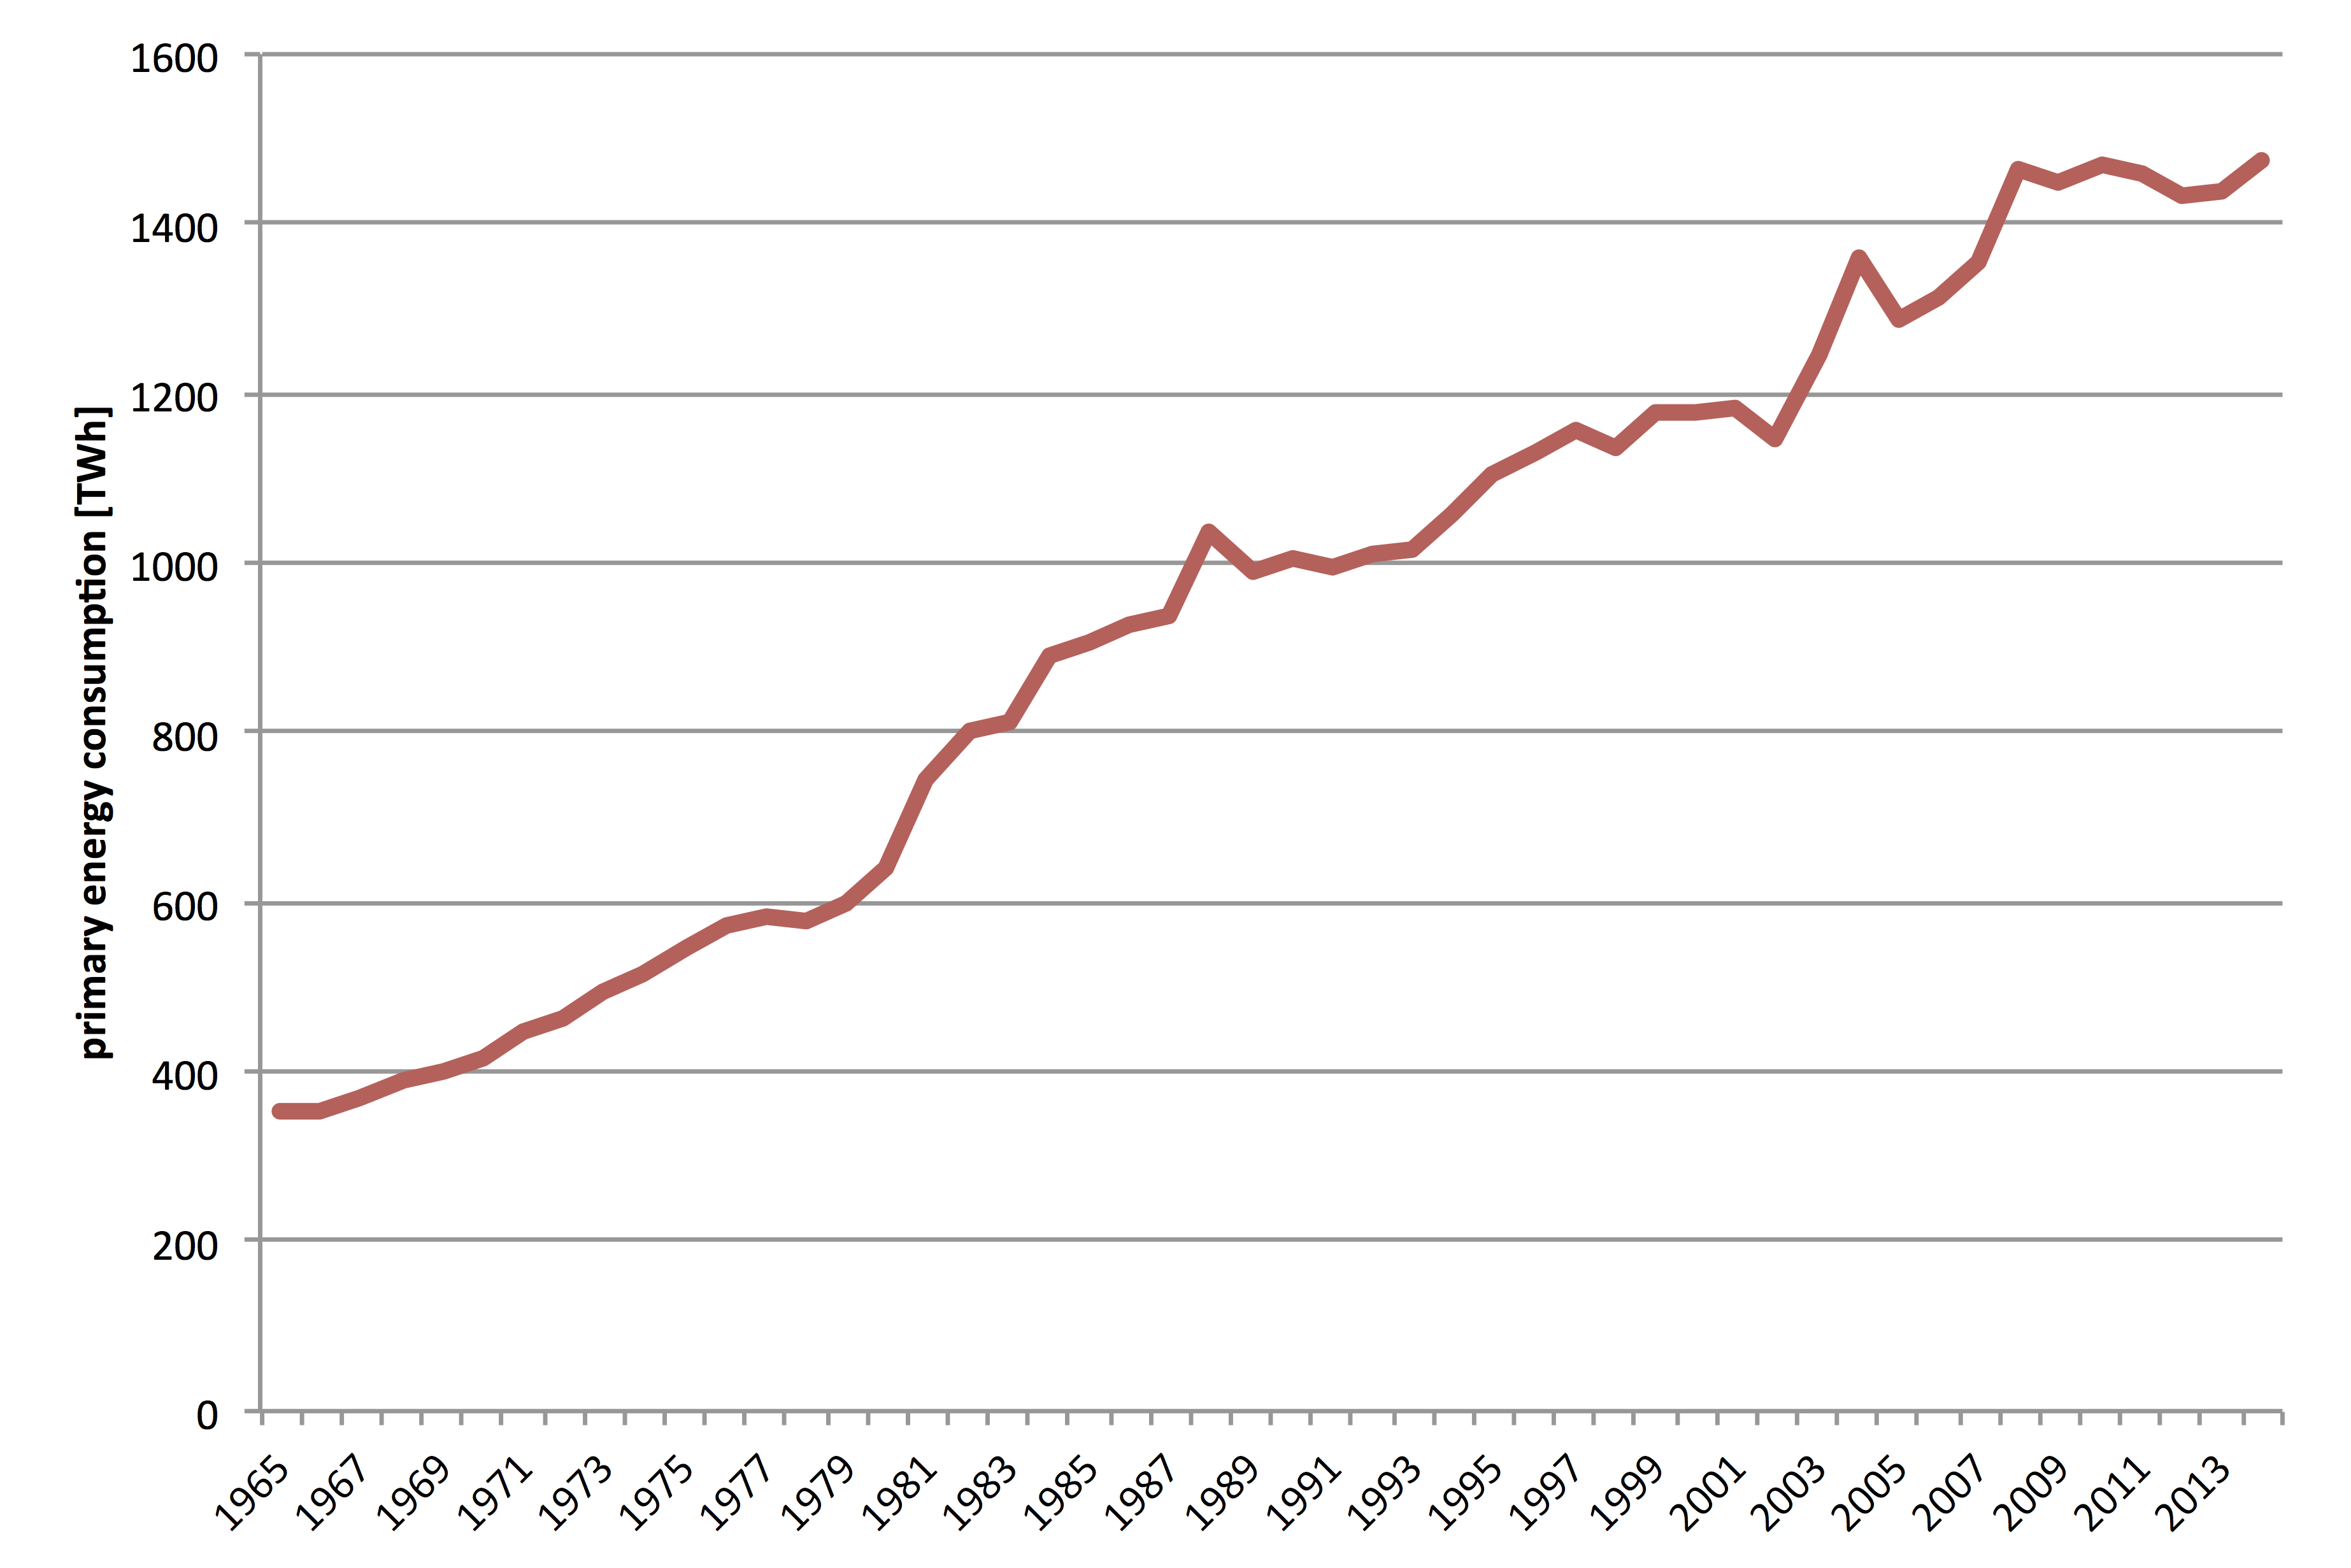
\includegraphics[width=1\linewidth]{FIG/PrimEnergyDevelopment}
\caption[Evolution of primary energy consuption of SA.]{Evolution of primary energy consuption of SA \cite{BP2015c}.}\label{PrimEnergyDevelopment}
\end{figure}
The spread in consumption of primary energy is defined by three major consumption groups, namly the industry sector with about 34.9~\%, the transport sector which consumes about 28.6~\% and other sectors with about 36.5~\%, which includes agriculture, commerce and public services, residential and non-specified consumers \cite{DepartmentofEnergy2012}. So it can be said that the sectors industy and transport are the main energy consumer in SA. 
\pagebreak
\section{Electricity supply and demand}
The electricity market in SA is regulated by the National Energy Regulator of South Africa (NERSA) in terms of the National Energy Regulatory Act from 2004. NERSA's area of responsibility includes the national grid codes, licences, provides, regulations of tariff increases and more. \cite{Eskom2015a}

SA has a fully state-owned and vertically integrated electricity supplier named Eskom (Eskom Holdings SOC Ltd.). Eskom supplies approximately 95~\% of SA's electricity and more than 45~\% of Africa \cite{EskomGenerationDivision2014}. In 2014 SA has a 1.1~\% share of the worldwide electricity consumption with a gross electricity output of 252.6~TWh \cite{BP2015c}. 92.6~\% of SA's primary energy consumption for electricity generation was based on coal fired power plants in 2013 and further 5.5~\% came by nuclear power plant \cite{Agency2015}. Therefore was Eskom in 2009 with 215.91~Mt~CO\textsubscript{2} also worldwide number five of the power companies with the highest CO\textsubscript{2} emissions \cite{CARMA2015}.

Figure~\ref{Electr} compares the South African and worldwide primary energy consumption for electricity generation in 2013. As it is shown, besides coal and nuclear based power generation makes just hydroelectric generation any significant part. \cite{Agency2015}

\begin{figure}[!htbp]
        \centering                
        \begin{subfigure}[b]{0.45\textwidth}
                \centering
                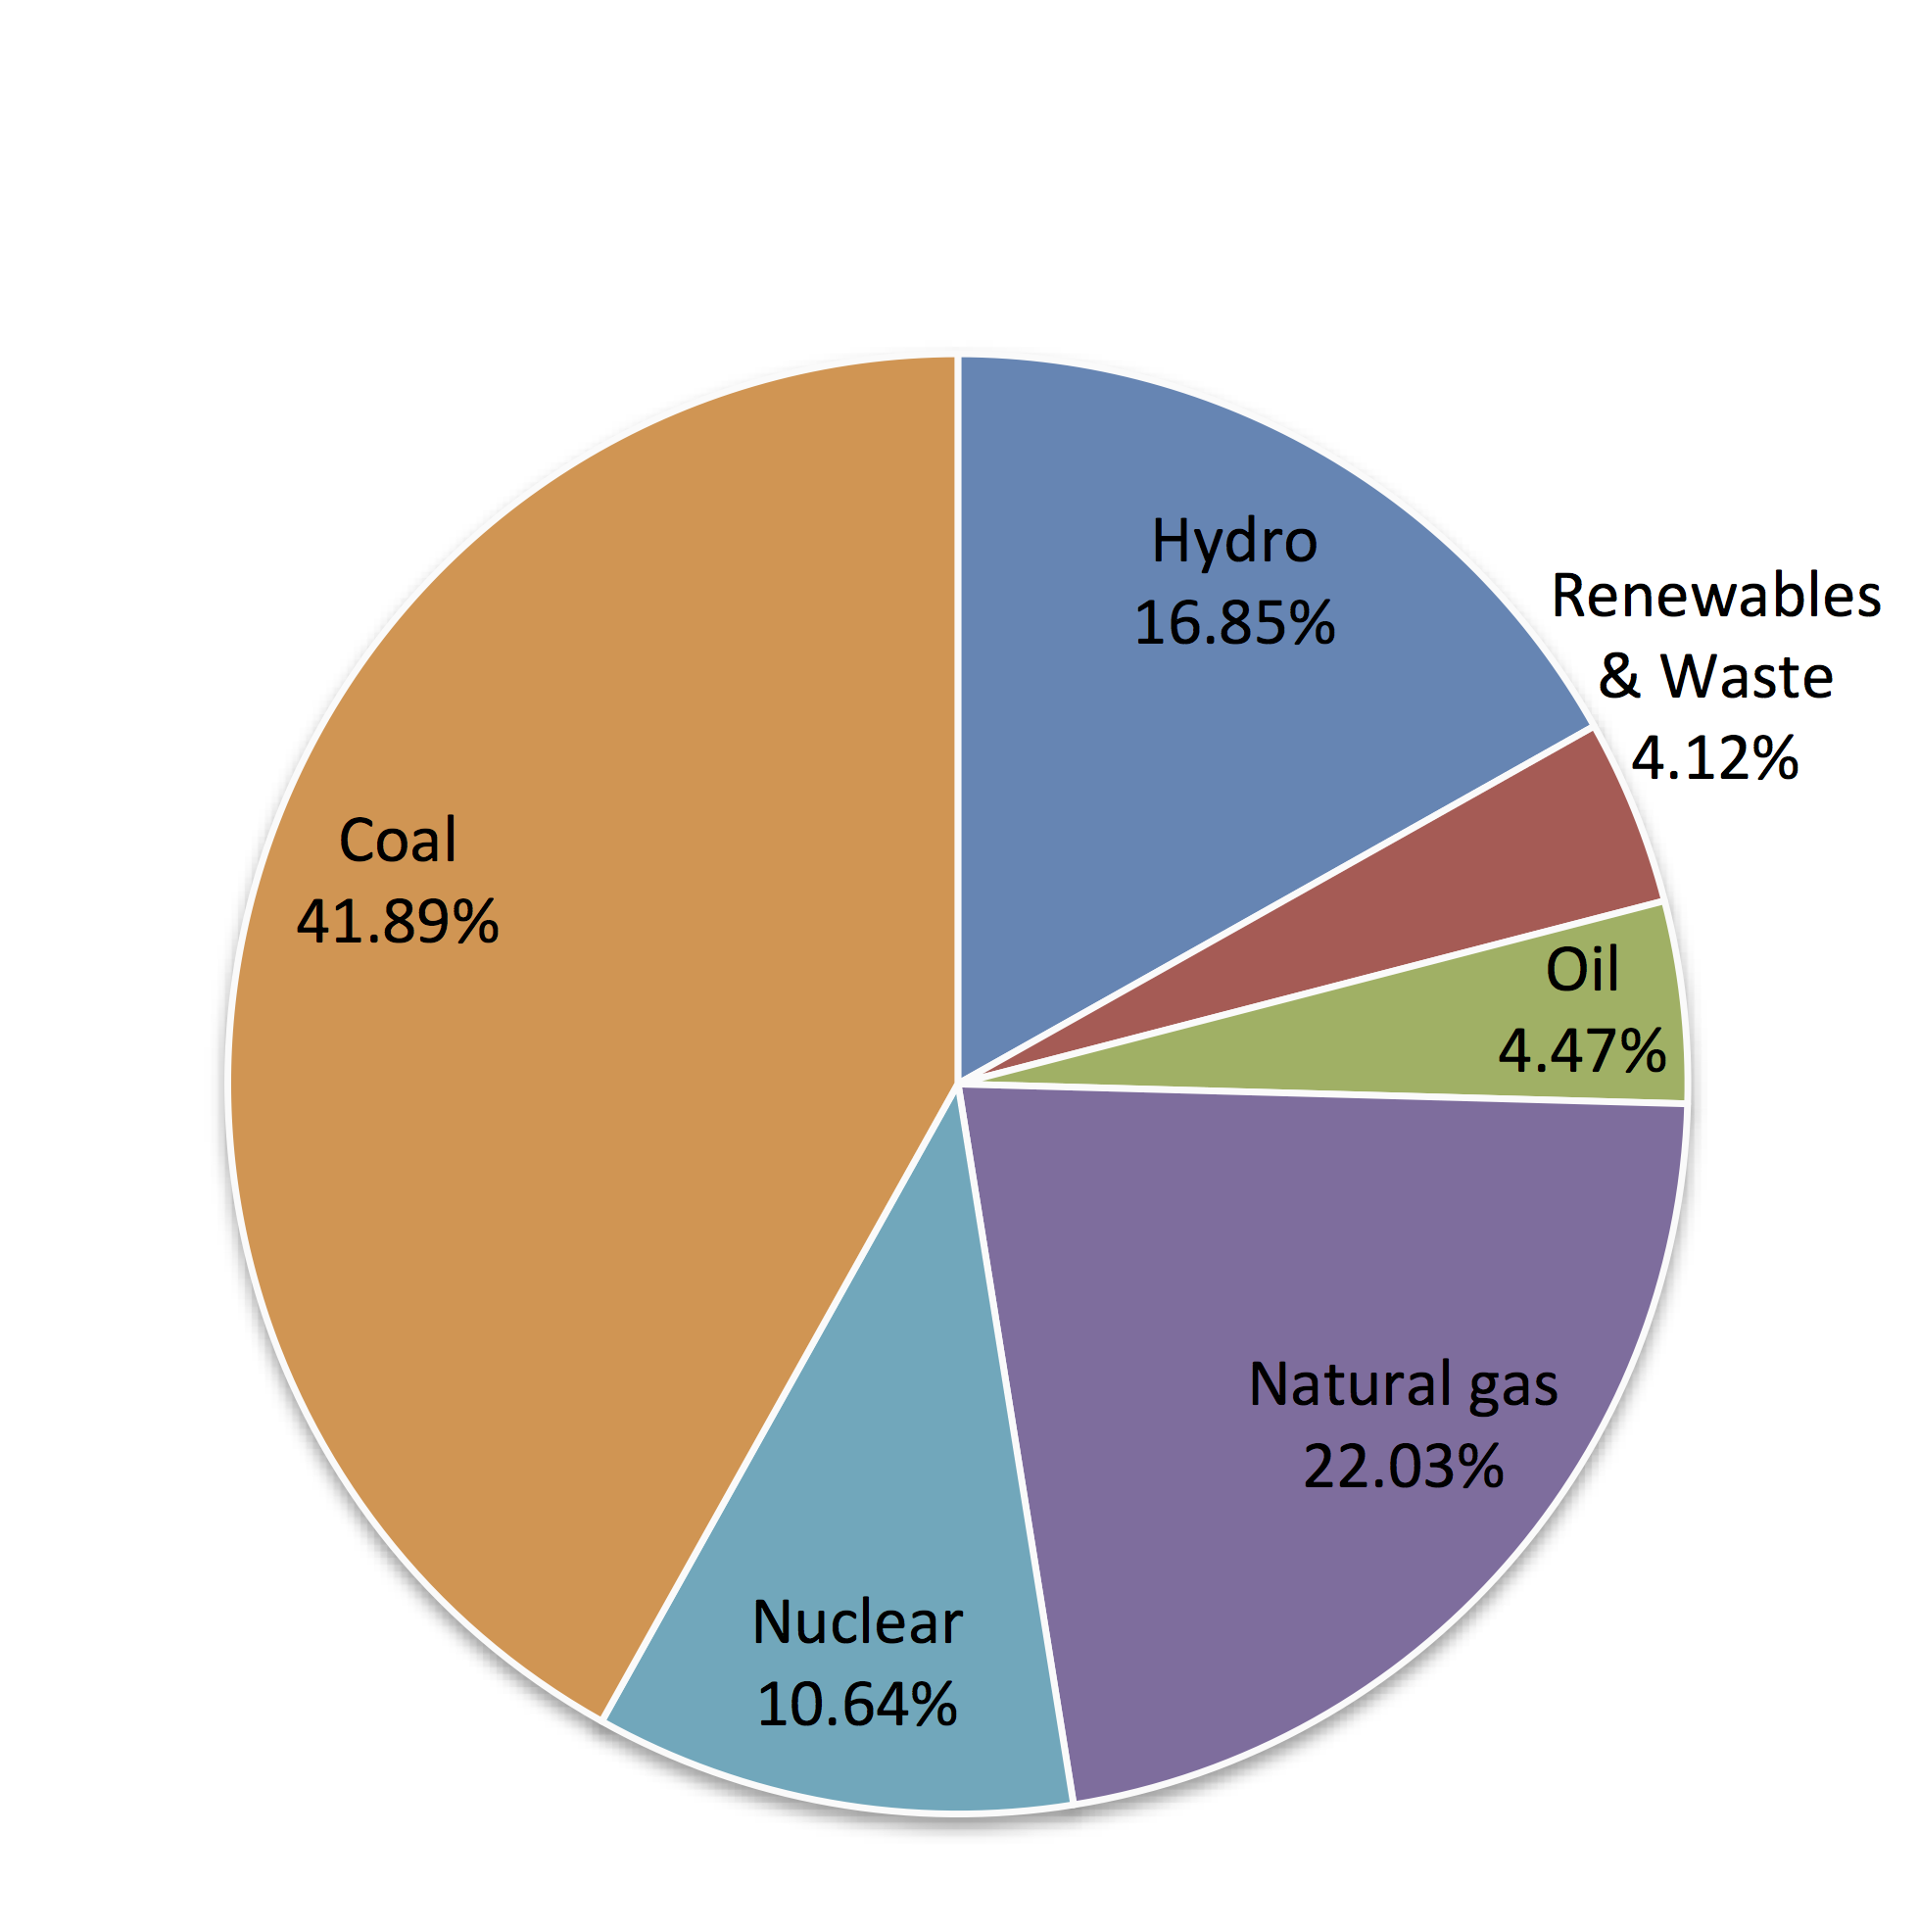
\includegraphics[width=1\textwidth]{FIG/ElectrWorld}
                \caption{World's allocation of primary energy consumption for electricity generation.}\label{ElectrWorld}
        \end{subfigure}
        ~
        \begin{subfigure}[b]{0.45\textwidth}
                \centering
                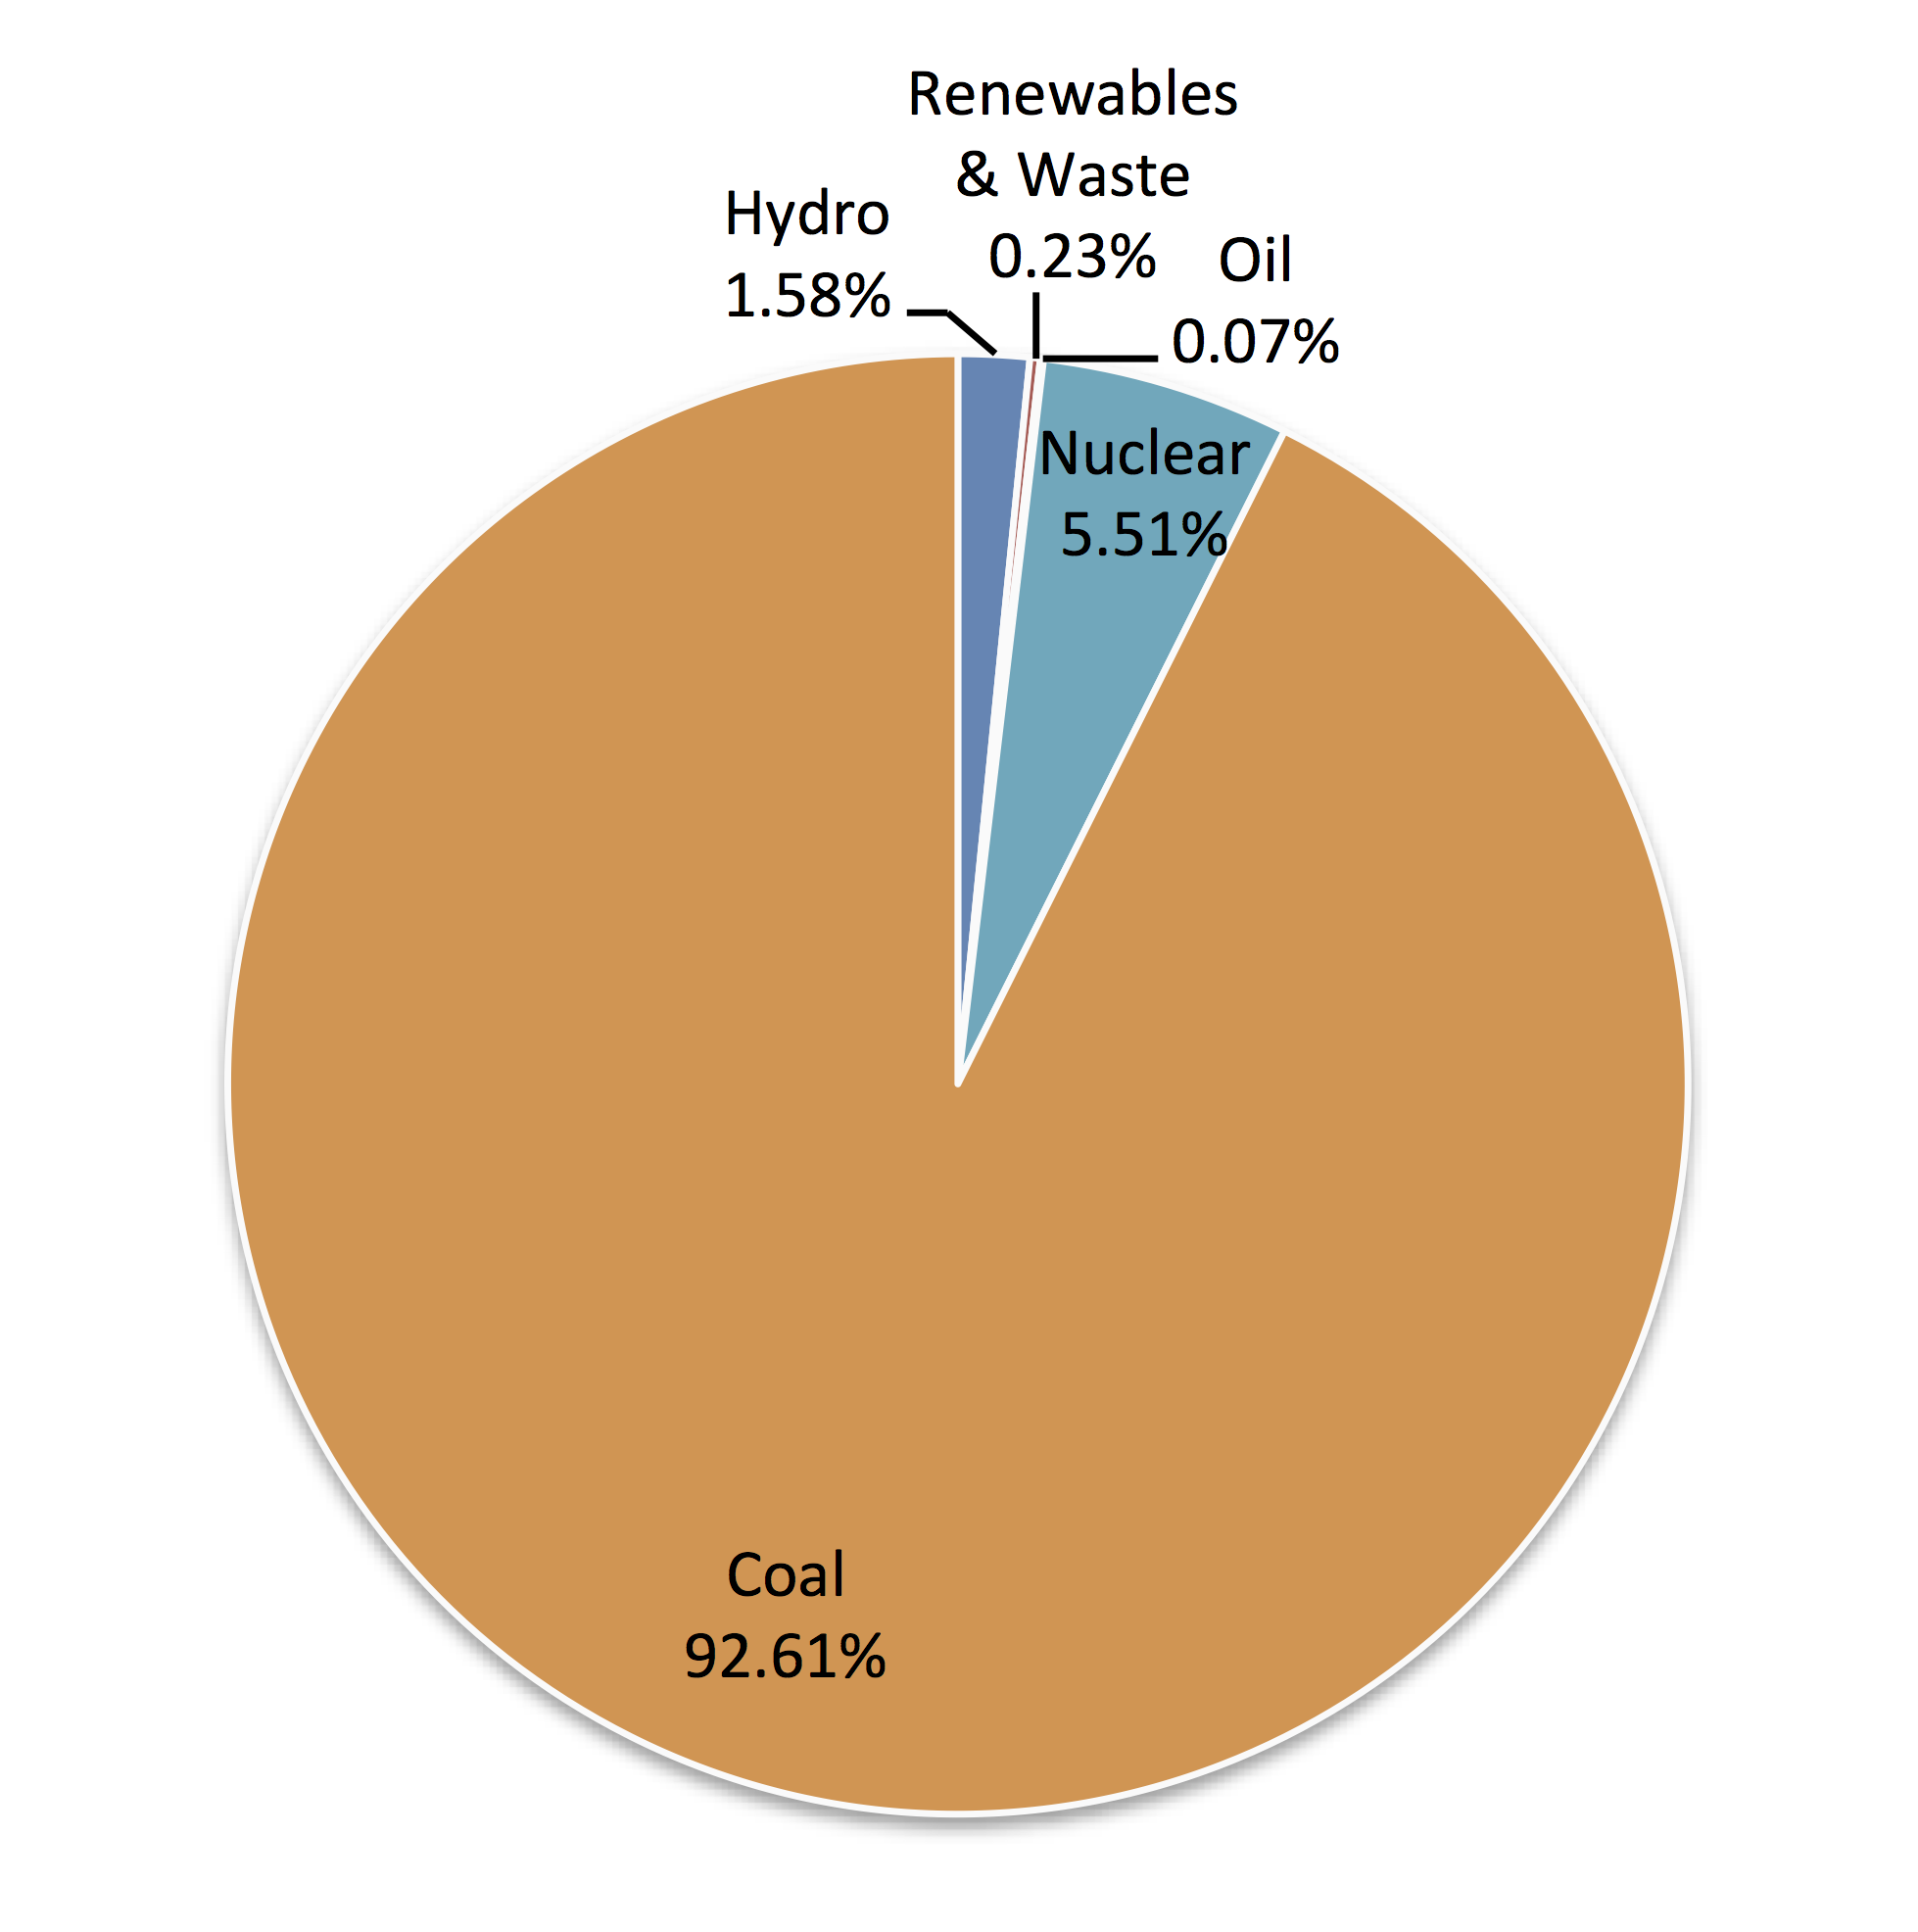
\includegraphics[width=1\textwidth]{FIG/ElectrSA}
                \caption{SA allocation of primary energy consumption for electricity generation.}\label{ElectrSA}
        \end{subfigure}
\caption[Comparision of primary energy consumption for electricity generation by fuel in 2013.]{Comparision of primary energy consumption for electricity generation by fuel in 2013 \cite{Agency2015}.}\label{Electr}
\end{figure}
As mentioned in 2014 the gross electricity generation was about 252.58~TWh in SA. But when taking an eye on the evolution of the gross electricity generation of the last three decades in Figure~\ref{electrGross} it can be noted that the generation peaked in 2007 with 263,48~TWh. \cite{BP2015c} 

\begin{figure}[htbp]  
\centering
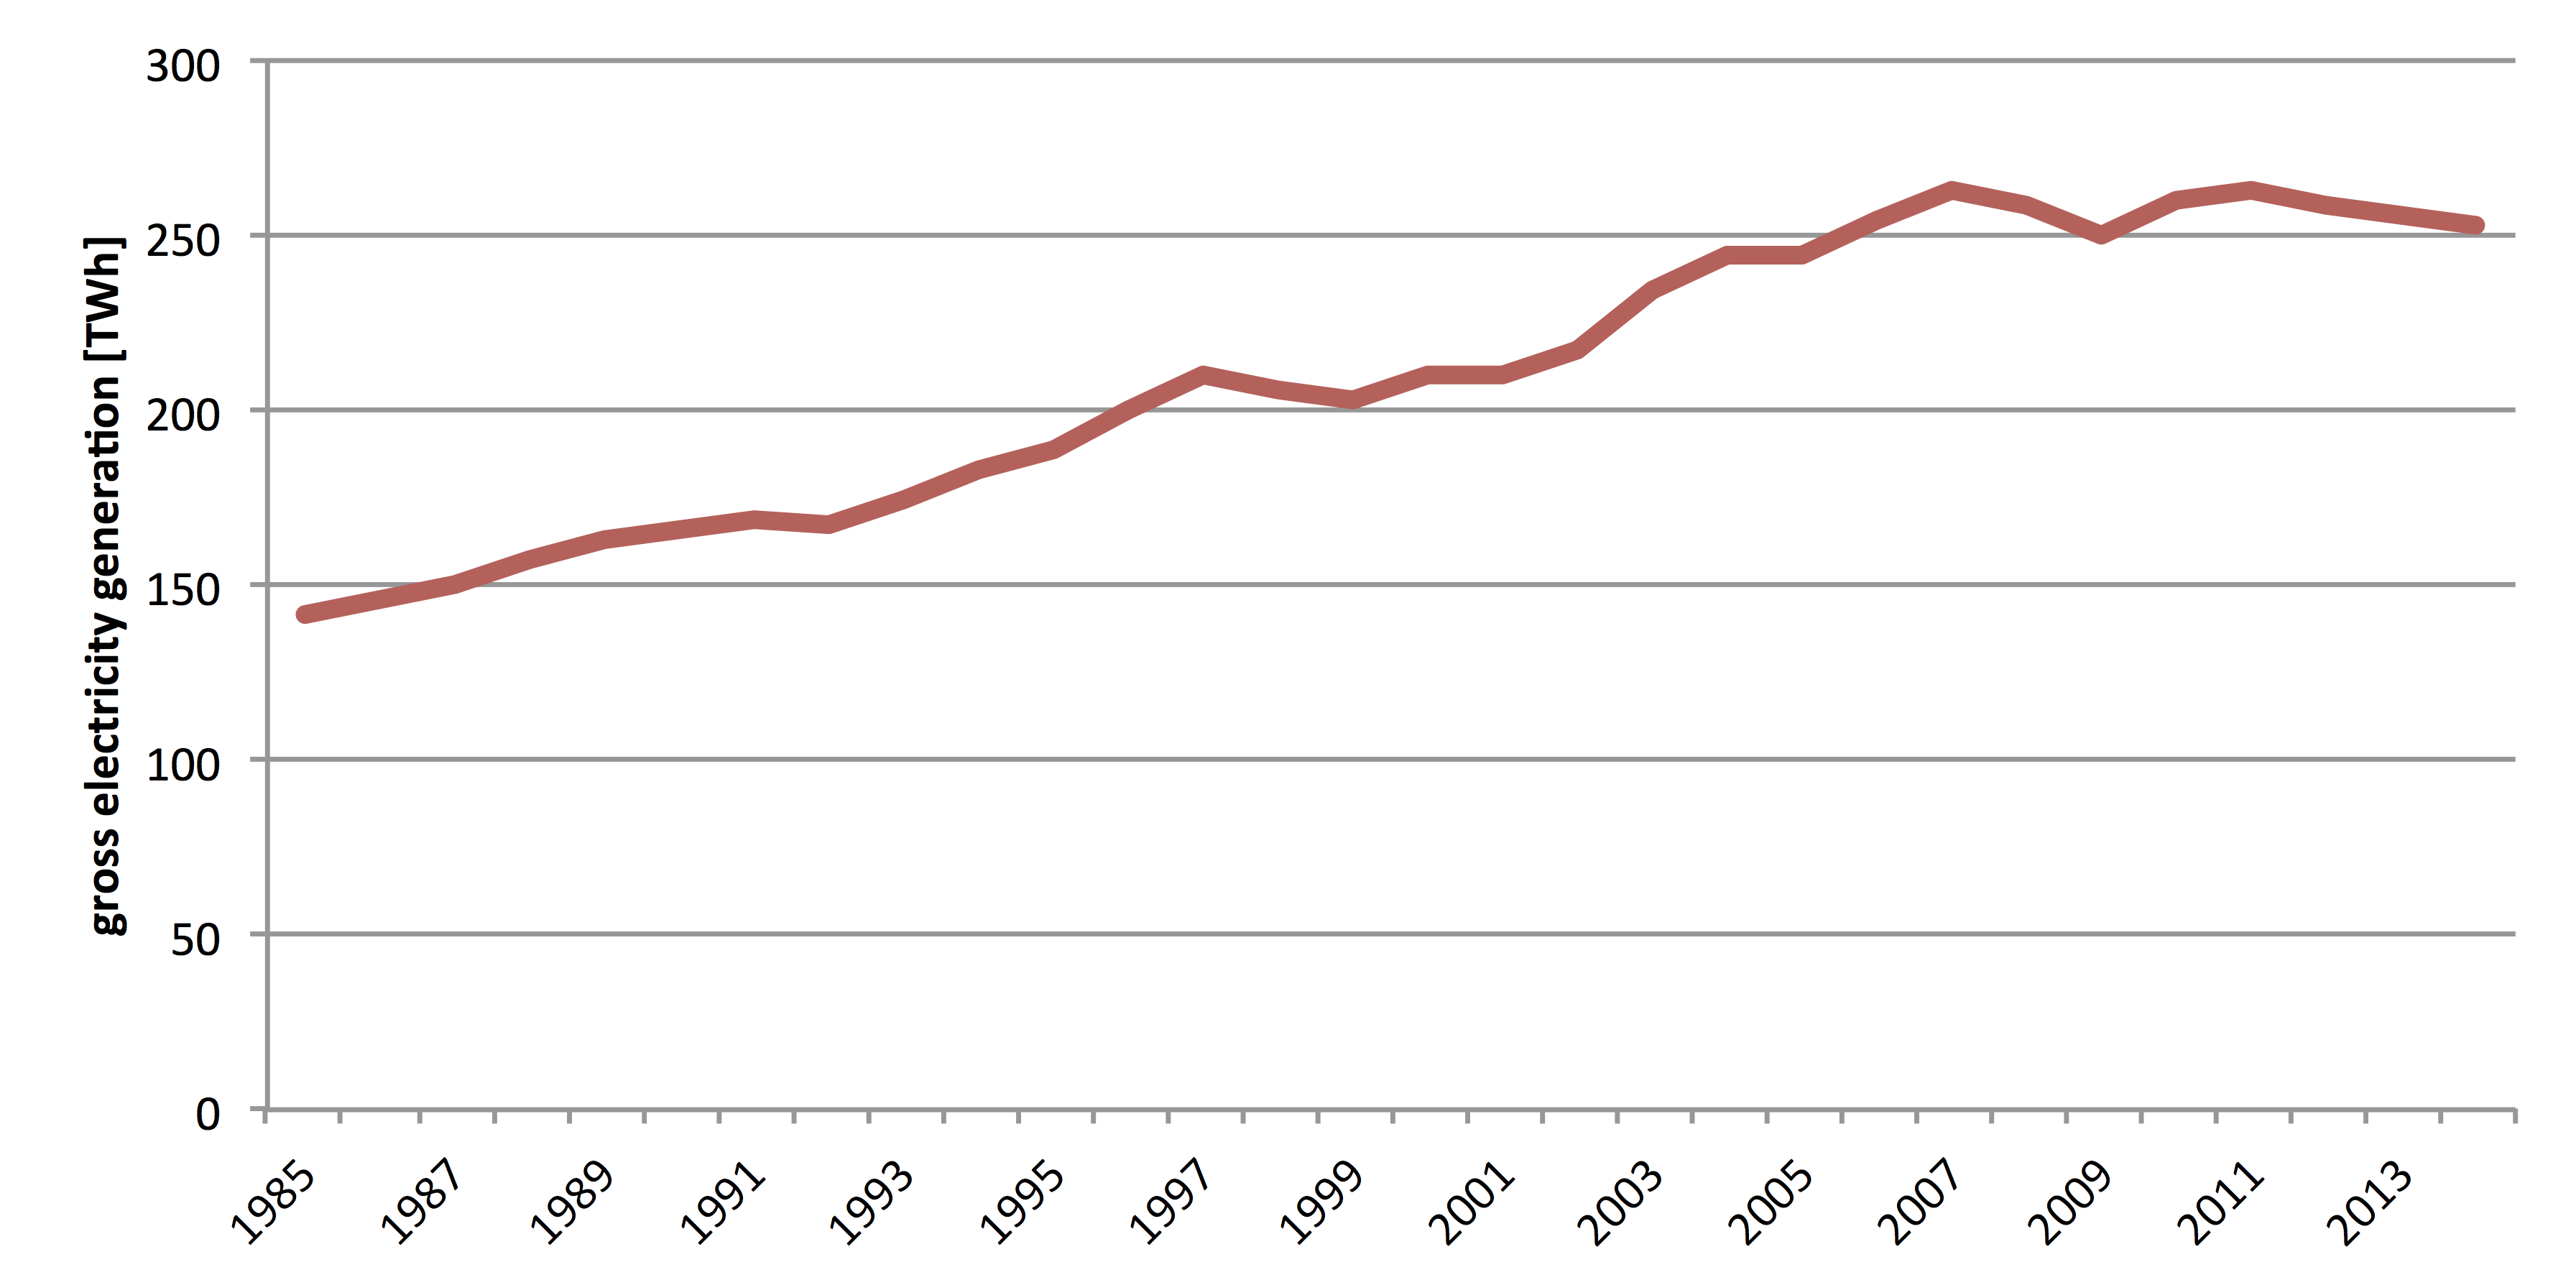
\includegraphics[width=1\linewidth]{FIG/electrGross}
\caption[Evolution of gross electricity generation in SA.]{Evolution of gross electricity generation in SA \cite{BP2015c}.}\label{electrGross}
\end{figure}
The leak on growth momentum of gross electricity generation in SA after the global financial crisis in 2009 is not leading from decreasing request in demand, but more from a power plant maintainence behind schedule and investment backlog. The delayed maintainence schedule was a results from Eskom's “keeping the lights on” philosophy what they are calling nowadays a "not sustainable approach" \cite{Eskom2014}. Eskom’s base load fleet has a average age of about 34 years with a plant availability of about 73~\% \cite{Eskom2015c}. This facts be associated with the rising annual unplanned capability loss factor (UCLF) of Eskom’s power plant fleet. Figure~\ref{UCLF} shows that the UCLF rises from 2008/09 on significantly. In 2014/15 the UCLF reached their maximum of 15.22~\%. The rising UCLF comes in hand with implementing of “load shedding” by Eskom in 2008, which is a planned rolling blackouts based on a schedule in order to protect the power system from a total blackout \cite{Eskom2015d}. Eskom implemted a load shedding schedule in four stages, wich allows Eskom at Stage 4 to dropping of up to 4~000~MW of the national load to balance electricity supply and demand. \cite{Eskom2015e}

\begin{figure}[htbp]  
\centering
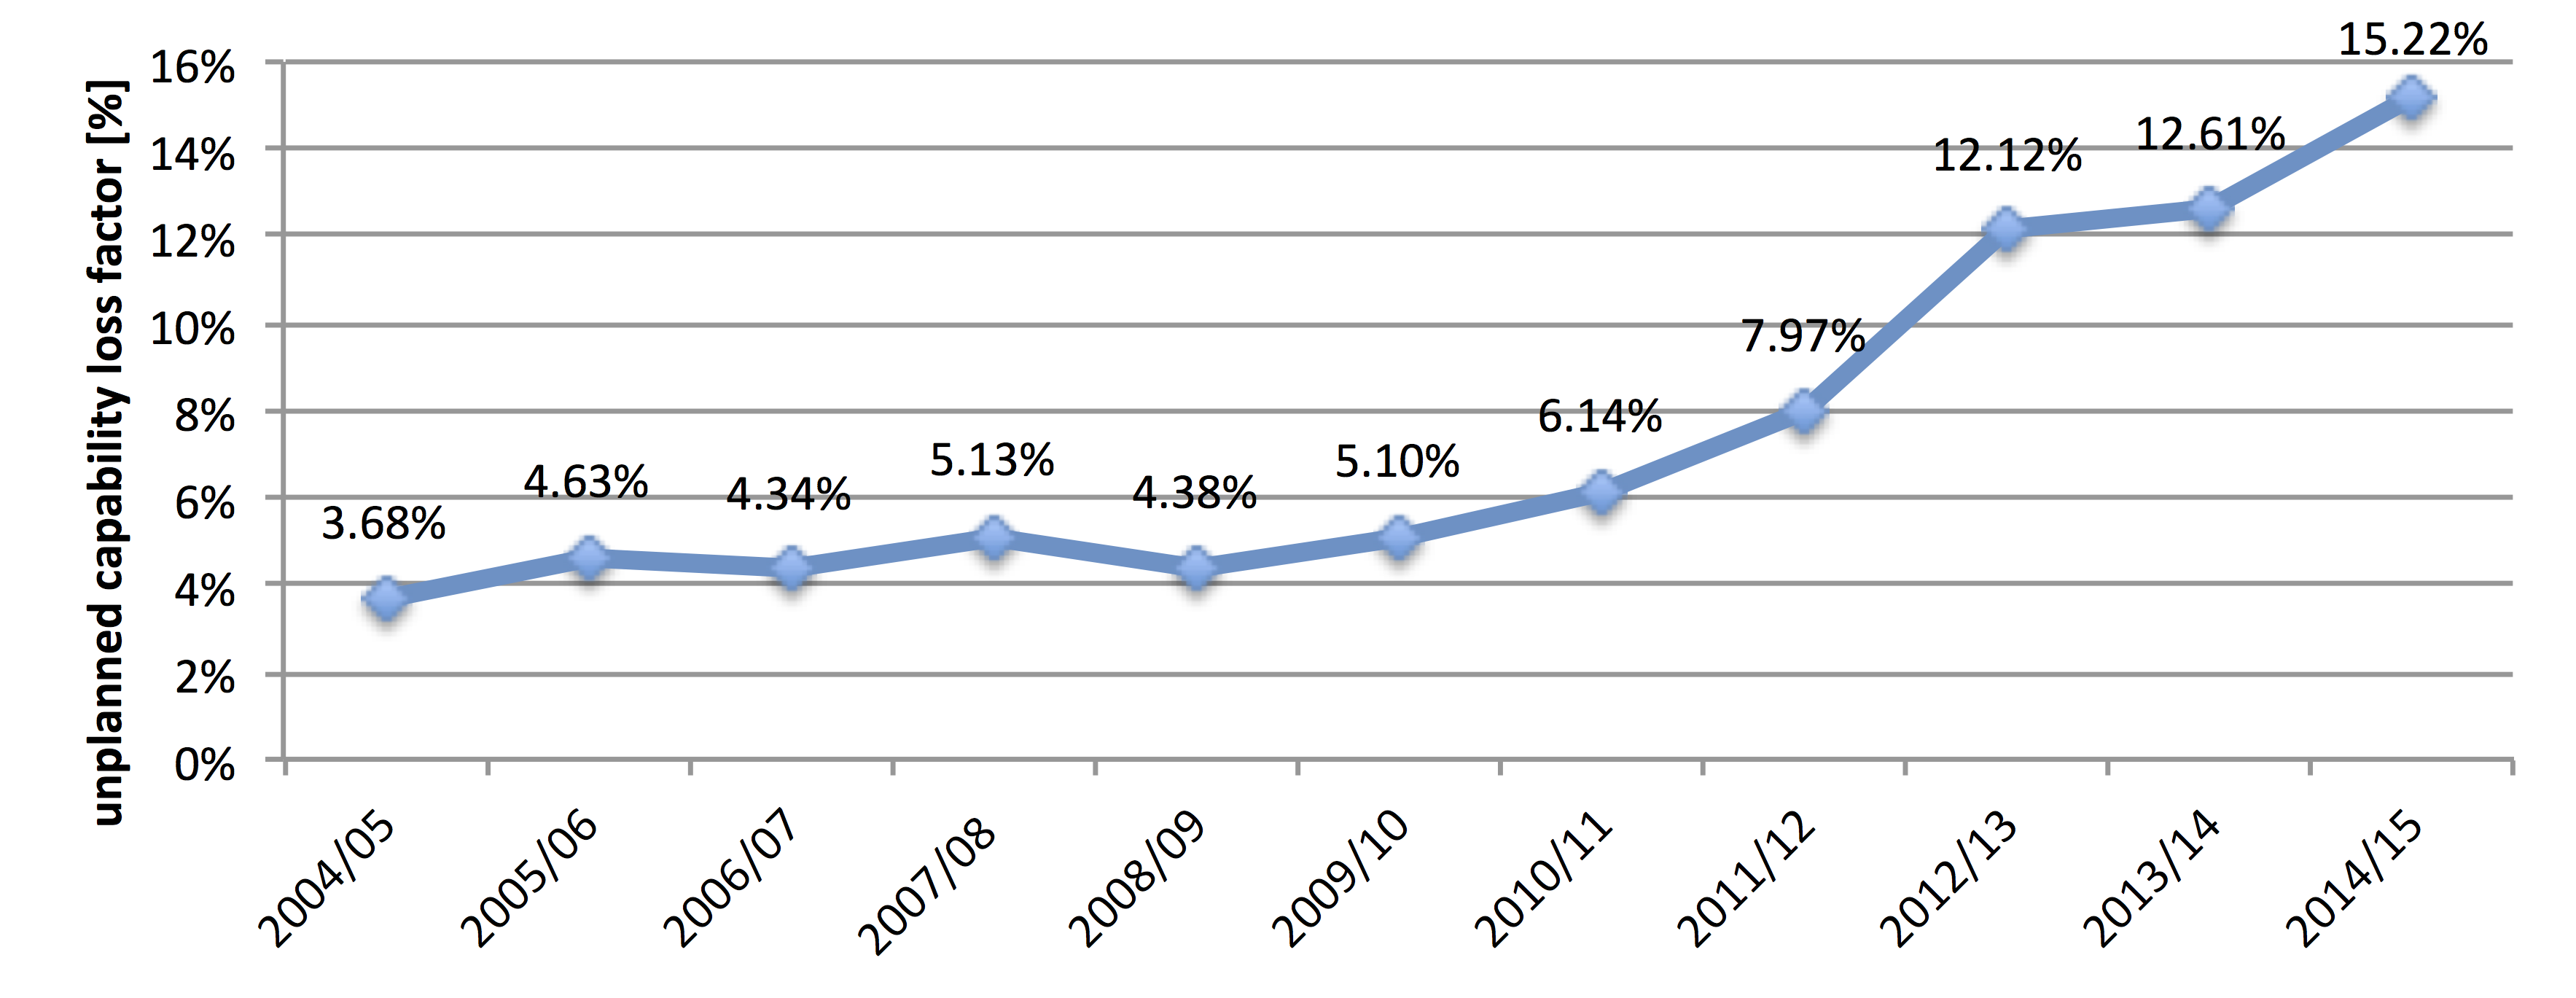
\includegraphics[width=1\linewidth]{FIG/UCLF}
\caption[Evolution of Eskom's annual unplanned capability loss factor.]{Evolution of Eskom's annual unplanned capability loss factor \cite{Eskom2015b,Eskom2015d}.}\label{UCLF}
\end{figure}
SA has currently a total nominal installed capacity of 45~699~MW, therefrom Eskom owns and manage 42~090~MW power station capacity in March 2015 \cite{Eskom2015b}. Almost 85~\% of Eskom's power plant capacity are coal-fired (35~721~MW), 4.4~\% nuclear (1~860~MW) and 5.7~\% gas-fired (2~409~MW) which is shown in Figure~\ref{PgenerationEskom}. Besides these fossil and nuclear based capacities Eskom owns also capacities in pumped storage (1~400~MW), hydro (600~MW) and wind (100~MW). Further 3~609~MW capacity coming from independent power producers (IPP) which also include 1~795~MW renewable generation trough the Renewable Energy Independent Power Producer Procurement Program (REIPPPP). \cite{Eskom2015a}

\begin{figure}[htbp]  
\centering
\includegraphics[width=0.45\linewidth]{FIG/PgenerationEskom}
\caption[Eskom's nominal installed power station capacity allocation in 2015.]{Eskom's nominal installed power station capacity allocation in 2015 \cite{Eskom2015a}.}\label{PgenerationEskom}
\end{figure}
The REIPPPP is one of the instruments that the SA Government uses to reaching there ambitious set target for a total installed capacity of 81~350~MW in 2030. From the aspired goal 17~430~MW are planed from wind and solar power. More precisely 9~770~MW by PV and 3~300~MW by CSP. \cite{DoE2013}

After five bid windows (incl. extended bid window in March 2014) the REIPPPP reached a committed capacity of 5~237~MW wherefrome 1~899~MW are commited to PV and 600~MW to CSP. \cite{DoE2015}

Currently most of the power generation is located in the north east of the country. Near to Johannesburg the capital of the province Gauteng are most of the country’s coal-fired power stations and coal mines allocated, as well as the country’s economic and industrial hub. SA is a country of wide open spaces and cities and towns are separated by large distance. Therefore long transmission lines are needed to transport electricity from the large power plants of the Gauteng province to the coastal areas. Figure~\ref{transmissionprojekts} gives an overview of the current situation of the allocations of the power stations and the transmission lines. Also Eskoms future transmission and power station projects are featured in the figure.

\begin{figure}[htbp]
\centering
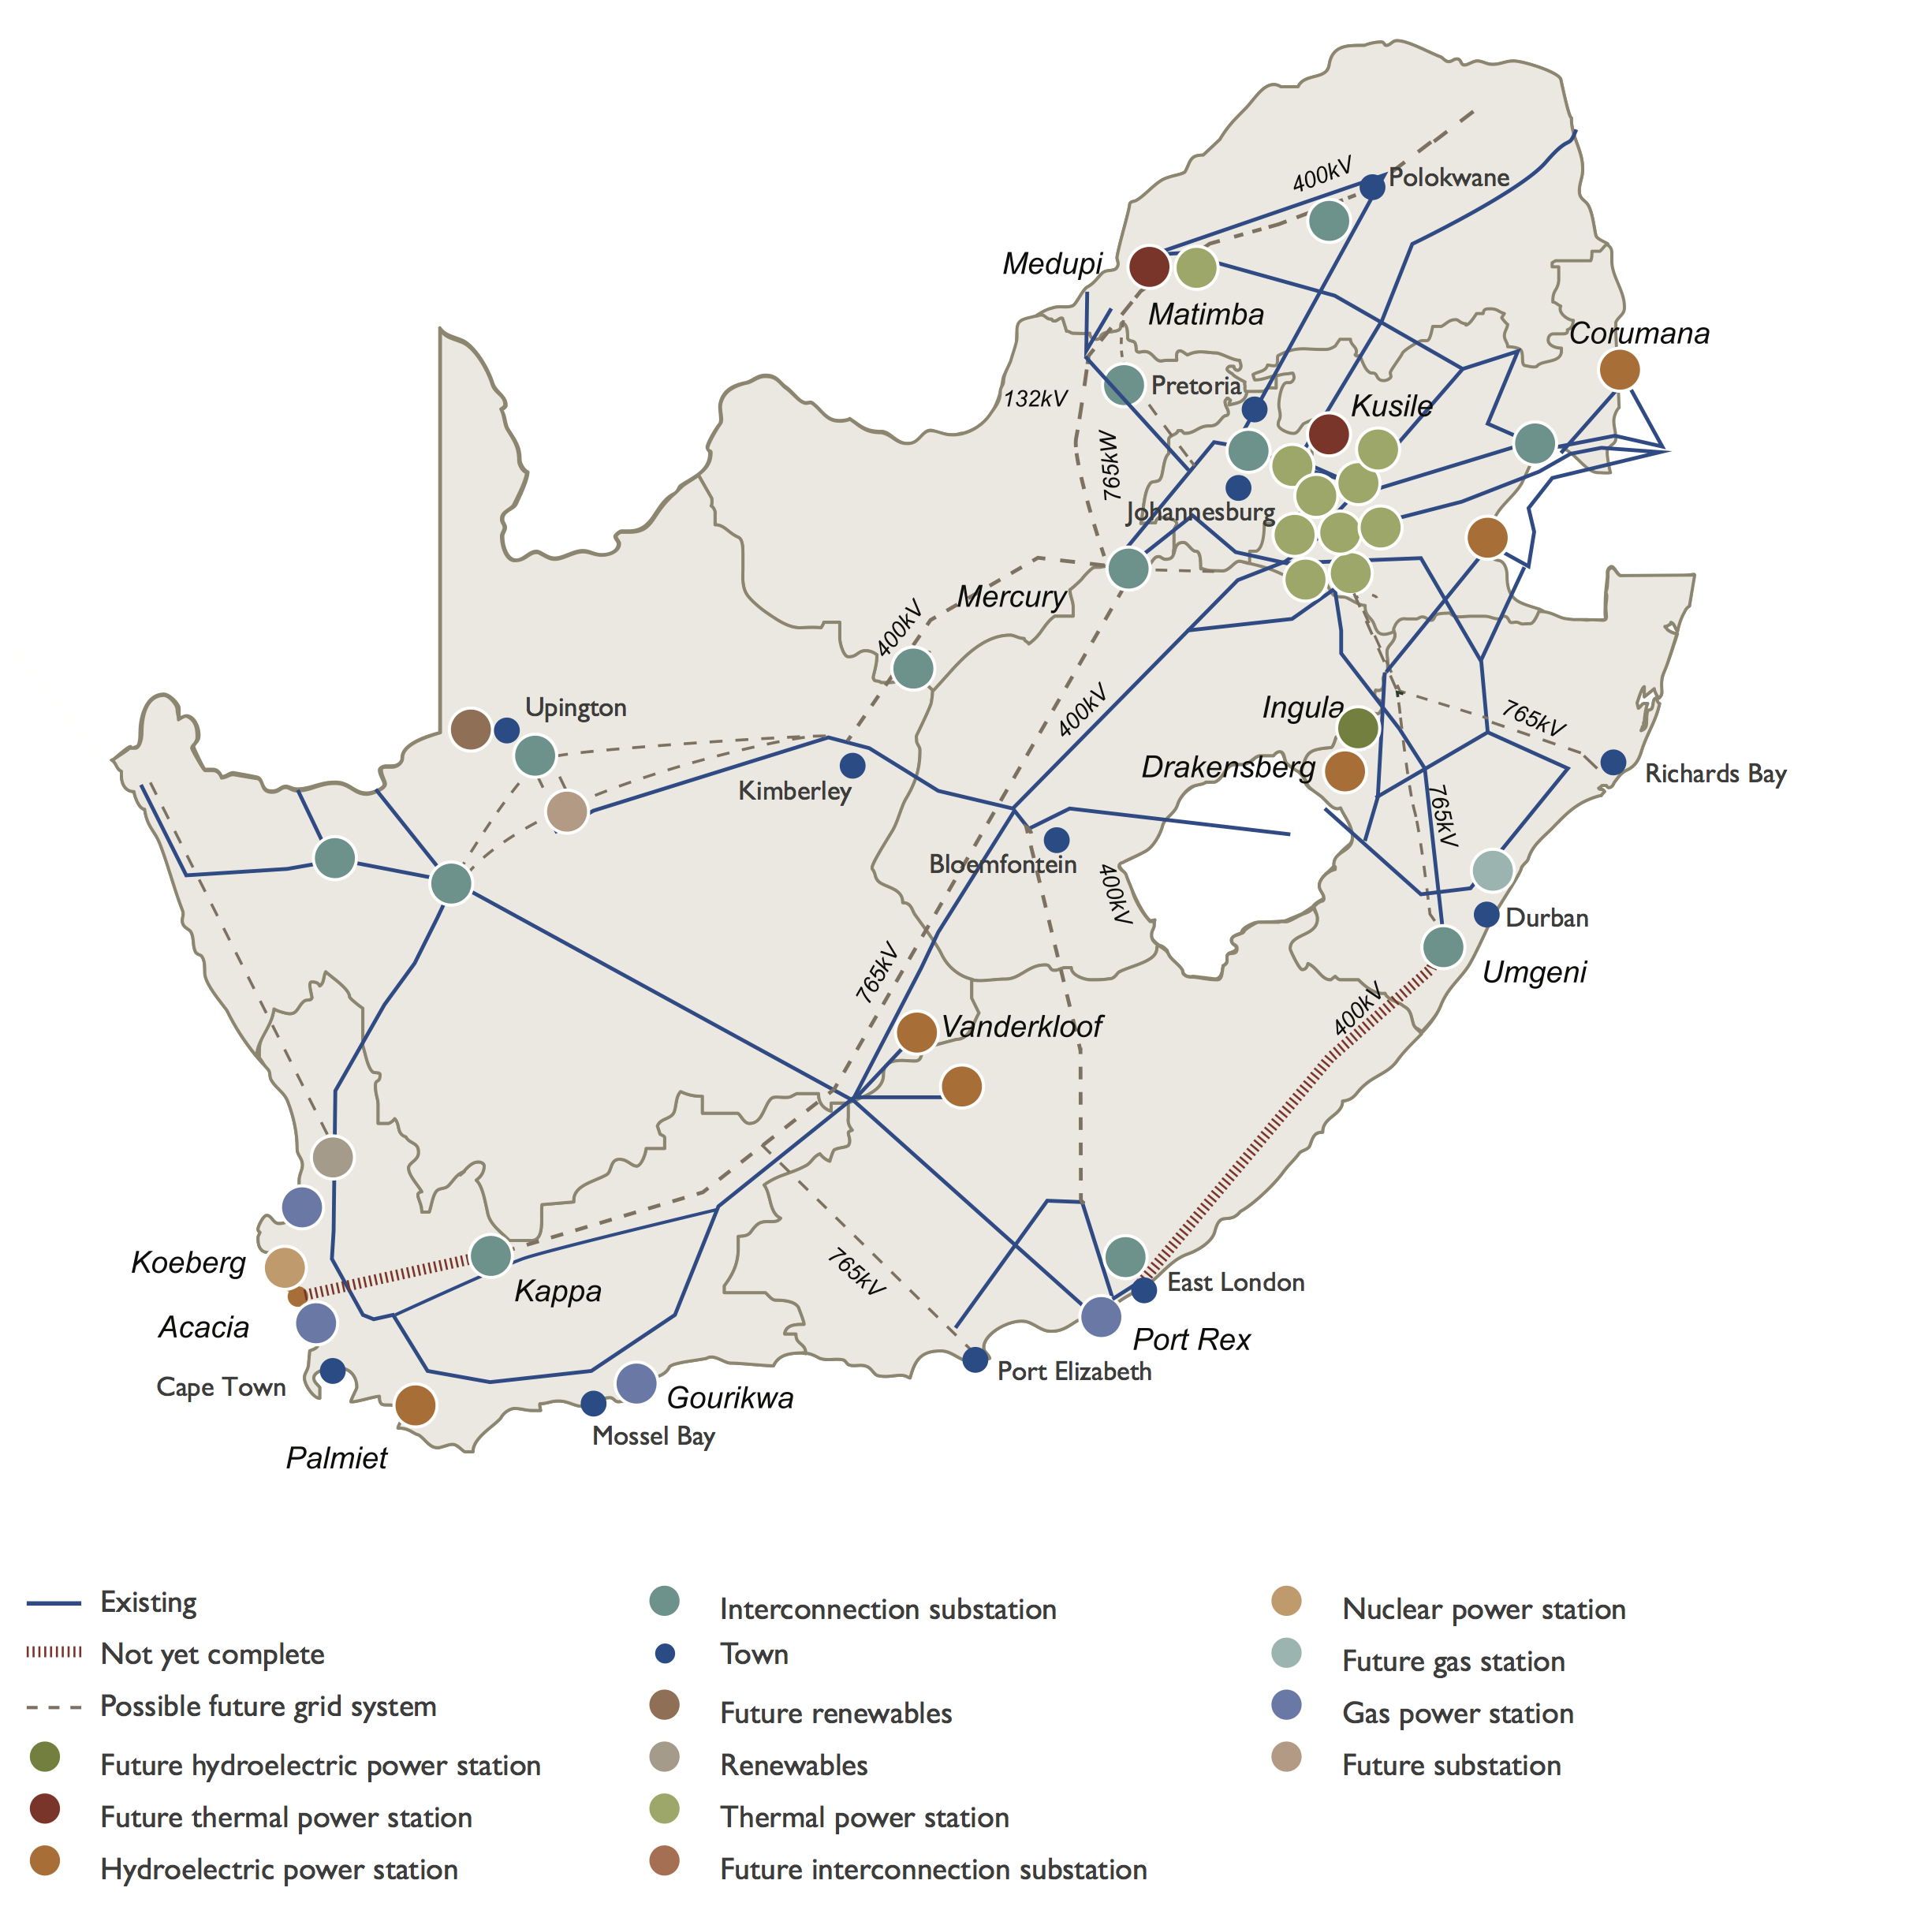
\includegraphics[width=1\linewidth]{FIG/transmissionprojekts}
\caption[Eskom’s transmission projects as at 31 March 2015.]{Eskom’s transmission projects as at 31 March 2015 \cite{Eskom2015a}.}\label{transmissionprojekts}
\end{figure}
Eskom operates, manages and maintains a total distance of 368~331~km power lines, whereof 31~107~km are transmission power lines at 765~kV to 132~kV and 48~278~km are distribution power lines at 132~kV to 33~kV. The residual power lines are 281~510~km reticulation power lines which are below 22kV and 7~436~km underground cables. Thereby is the country's total transformer capacity 239~490~MVA. The whole power supply system is controlled to a frequency of 50~Hz. \cite{Eskom2015b}

When taking again an eye on Figure~\ref{transmissionprojekts} it can be noted, that the area of Upington in the Northern Cape province is not yet accessed with high voltage transmission lines. Considering that the area of Upington provides the country’s highest solar irradiation value and is therefore a highly attractive site for solar power plants, new high voltage transmission lines to regions with higher load factors are necessary and are currently in its planning phase. Eskom is currently planing additional 3~940~km  transmission lines and 12~815~MVA transformer capacities till 2021 \cite{Eskom2015a}.

Through this electricity network SA covers a electrification rate of around 85~\% and which is the highest on mainland sub-Saharan Africa. About 11~\% of households don't have access to electricity and a further 4~\% rely on illegal access (non-paying) or obtain access informally (from one household to another but paying). \cite{IEA2014f}

In the financial year 2014/15 Eskom sales about 216~274~GWh. The spread of the main customers is shown in Figure~\ref{ElectricityShare}. From this it appears that the Municipalities are Eskom's biggest consumers. But also the Industrial and Mining sector makes together a considerable part of 38.6~\% of the electricity consumption. The residential part of the electricity consumption was just about 5.36~\% and the commercial part was below 5~\%. The main part of the exported electricity with about 70~\% went to the neighboring country Mosambique and further 10~\% to Botswana. Namibia and Swaziland mades just 8 or 7~\% of the exported electricity. \cite{Eskom2015b}  
\begin{figure}[!h] 
\centering
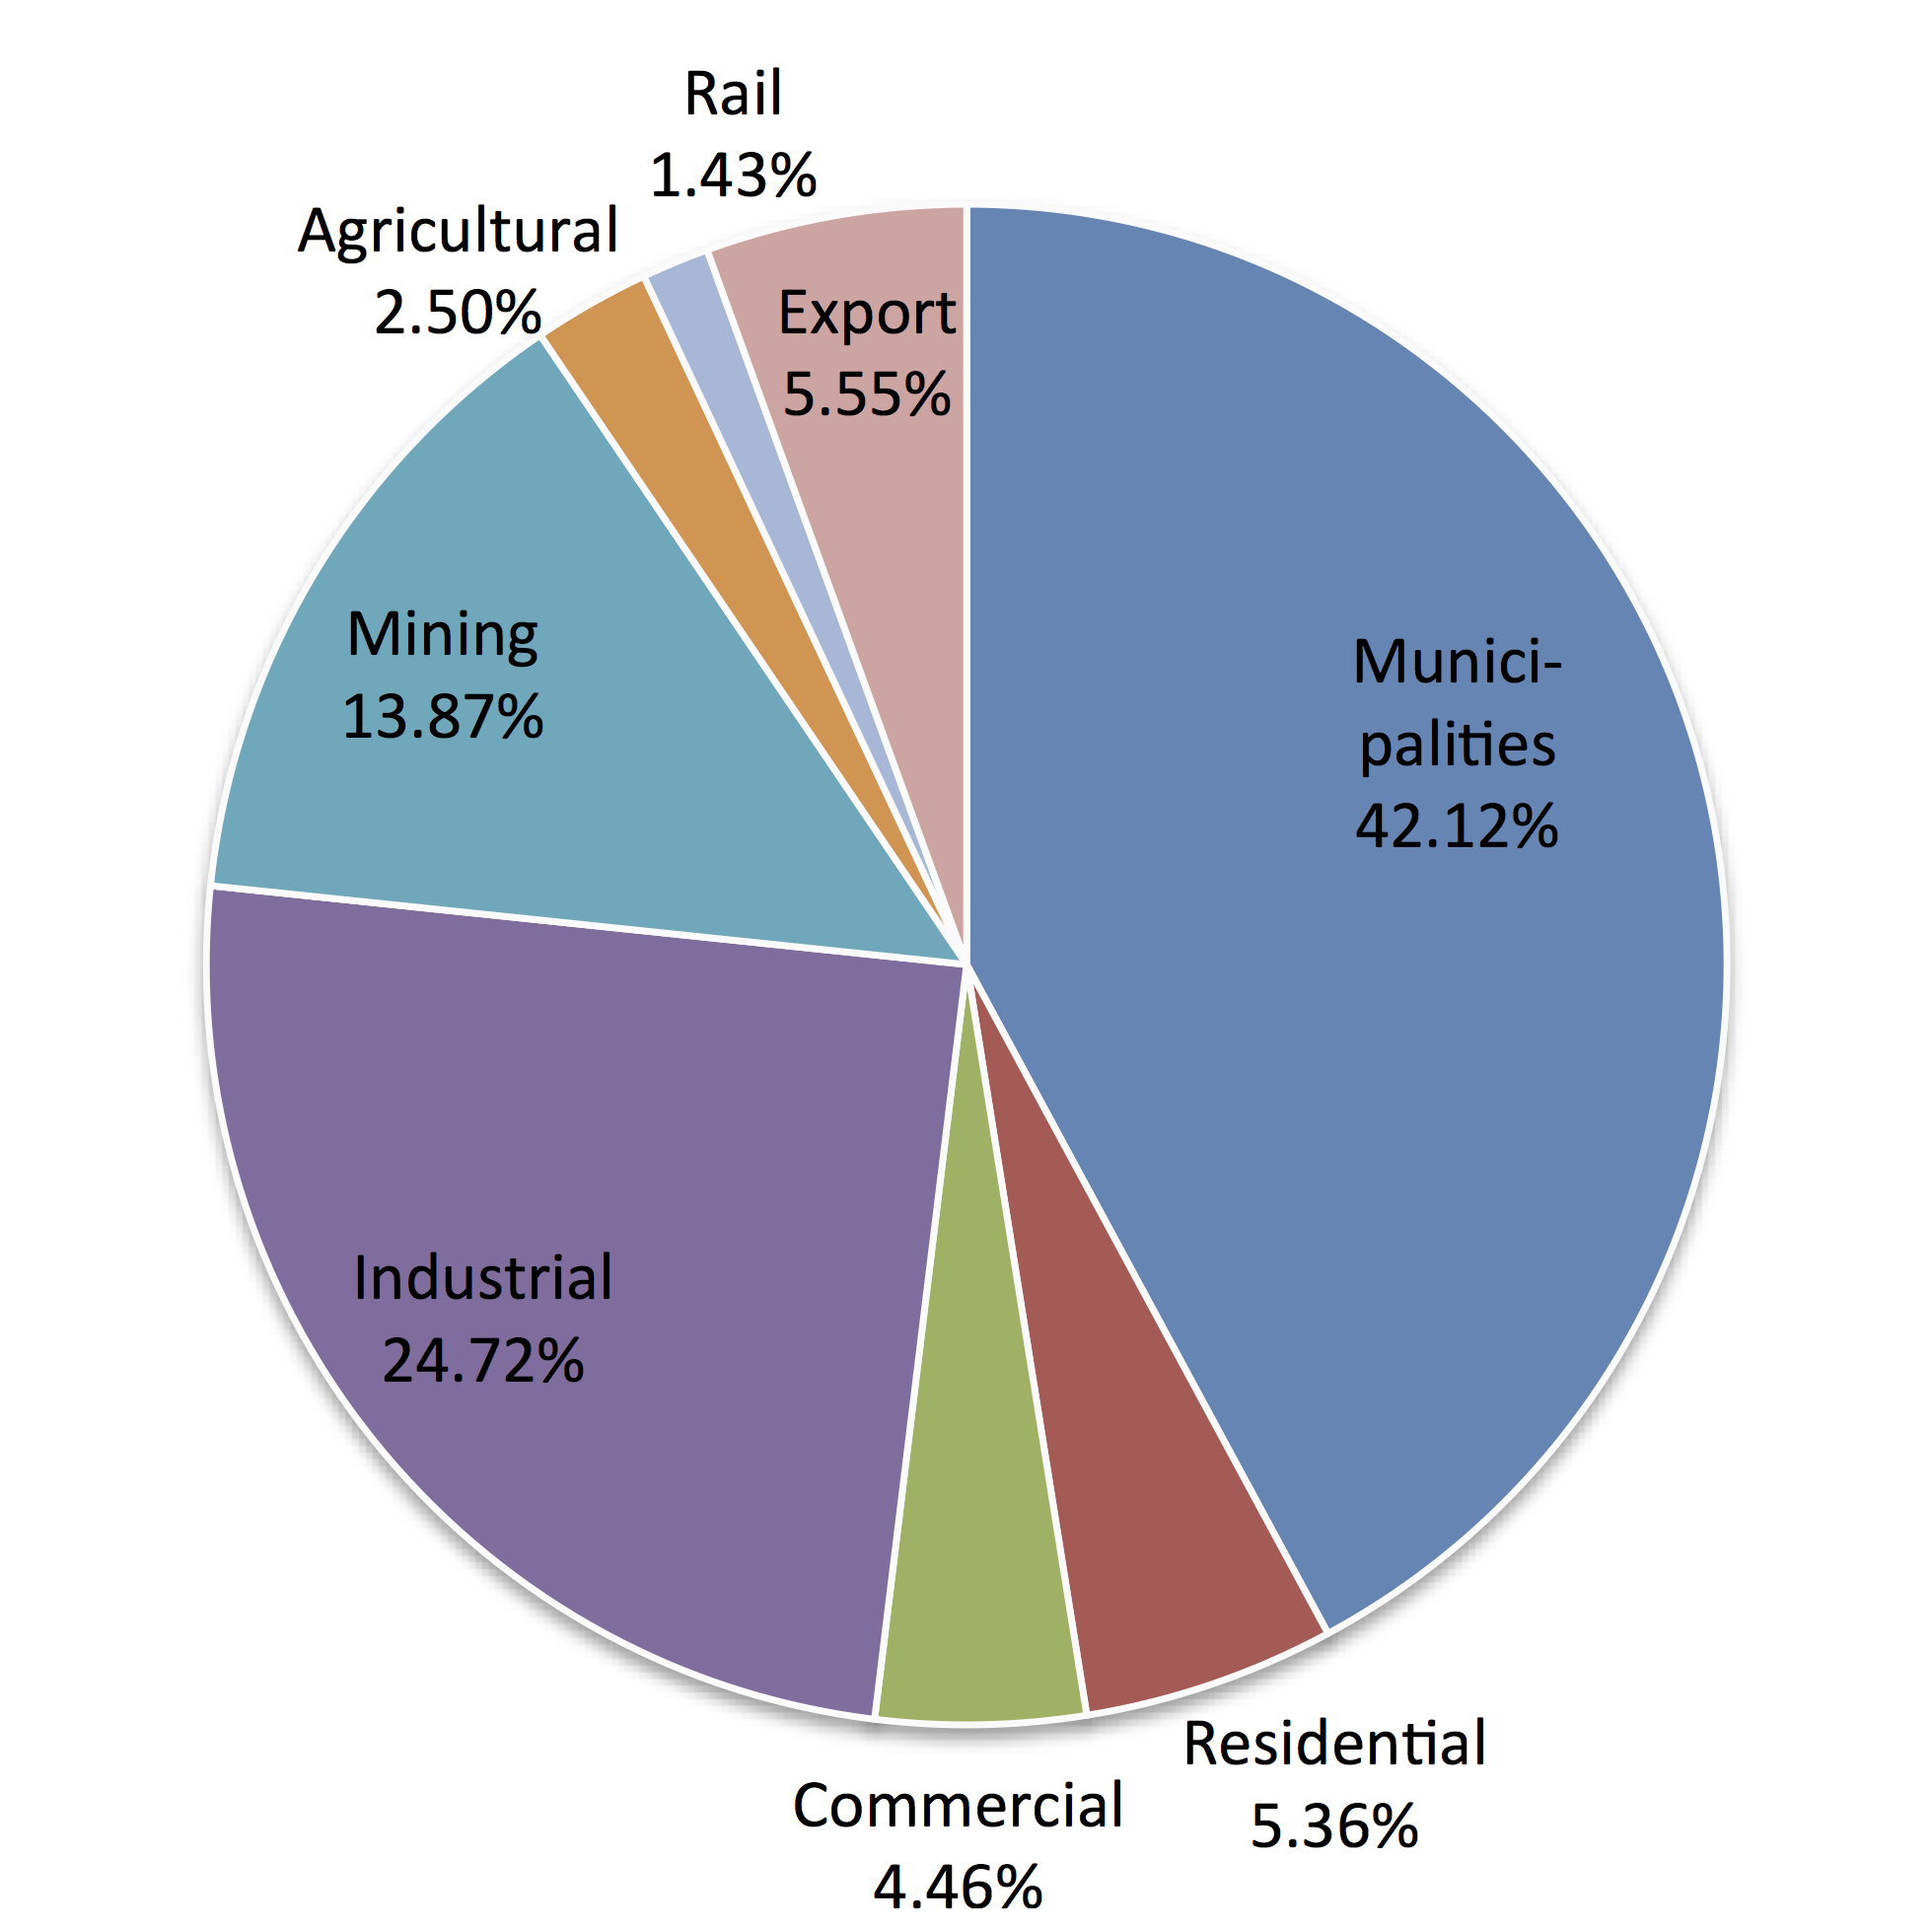
\includegraphics[width=0.4\linewidth]{FIG/ElectricityShare}
\caption[Eskom's electricity sales per customer category.]{Eskom's electricity sales per customer category \cite{Eskom2015b}.}\label{ElectricityShare}
\end{figure}
\pagebreak
